\documentclass[11pt]{article}
\usepackage{fullpage}
\usepackage{clrscode3e}
\usepackage{amsmath,amsthm,amssymb}
\usepackage{color}
\usepackage[shortlabels]{enumitem}
\usepackage{multicol,multirow}
\usepackage{csquotes}
\usepackage[super]{nth}


\usepackage{tikz}
\usepackage{pgfplots}
\usepgfplotslibrary{ternary, units}
\usetikzlibrary{decorations.pathmorphing, pgfplots.ternary, pgfplots.units}

\setlength{\parskip}{2mm}
\setlength{\parindent}{0mm}

\newcommand{\titlebox}[3]{
    \begin{center}
        \framebox{
            \vbox{
            \hbox to \textwidth { #1 \hfill #3}
            \vspace{-4mm}
            \hbox to \textwidth {\hfill \Large \bf #2 \hfill}
        }
    }
    \end{center}
}

\renewcommand*\arraystretch{1.5}

\newcommand\abs[1]{\left|#1\right|}

\newcommand{\answer}[1]{
\vspace{.5\baselineskip} \hrule \vspace{.5\baselineskip}
#1
\vspace{.5\baselineskip} \hrule \vspace{.5\baselineskip}
}


\usepackage{xcolor}

\definecolor{Green}{rgb}{0,0.7,0}
\definecolor{Purple}{rgb}{0.6,0,0.7}
\definecolor{Pink}{rgb}{1,0.33,0.64}


\newcommand\red[1]{\textcolor{red}{#1}}
\newcommand\blue[1]{\textcolor{blue}{#1}}
\newcommand\green[1]{\textcolor{Green}{#1}}
\newcommand\one{\red{1}}
\newcommand\two{\blue{2}}
\newcommand\three{\green{3}}
\newcommand\nat{\textcolor{violet}{N}}
\newcommand\purple[1]{\textcolor{Purple}{#1}}
\newcommand\paystwo[2]{\red{#1},\blue{#2}}
\newcommand\paysthree[3]{\red{#1},\blue{#2},\green{#3}}



\begin{document}

\titlebox{CSC 383, S'23}
{Homework 9}
{Due May \nth{3}}

\textbf{Directions:}

Write your solutions using and \LaTeX.
Then submit the files \texttt{hw9.tex}, \texttt{hw9.pdf}, and \texttt{tic-tac-toe.ipynb}.





\subsection*{Problem 1}

\begin{enumerate}[(a)]

\item
Use the Jupyter notebook \texttt{tic-tac-toe.ipynb} to prove that tic-tac-toe is a draw.
There is a node class already implemented for you that represents a state of the game for tic-tac-toe.
Your task is to implement backwards induction and use it to demonstrate that both players get utility zero in the subgame perfect equilibrium.

\item
Briefly explain how you know that when your code finds one SPE with utility 0, it means every SPE of tic-tac-toe must result in a draw.
\textbf{Hint:} think about what theorem from earlier in the semester helps answer this question.

\answer{

The Mini-Max theorem states that every Nash equilibrium is both a max-min and min-max for each player in a zero-sum game.  We found one sub-game perfect equilibrium with utility zero.  We also know that every sub-game perfect equilibrium is a Nash equilibrium.  So, by the Mini-Max theorem, every Nash equilibrium must be zero, and in this case, every sub-game perfect equilibrium gives a utility of 0.

}

\end{enumerate}



\subsection*{Problem 2}

Use the extensive form game tree for Kuhn poker, and the following cumulative gains so far to perform the next iteration of the CFR algorithm.

{\small
\hspace{-14mm}
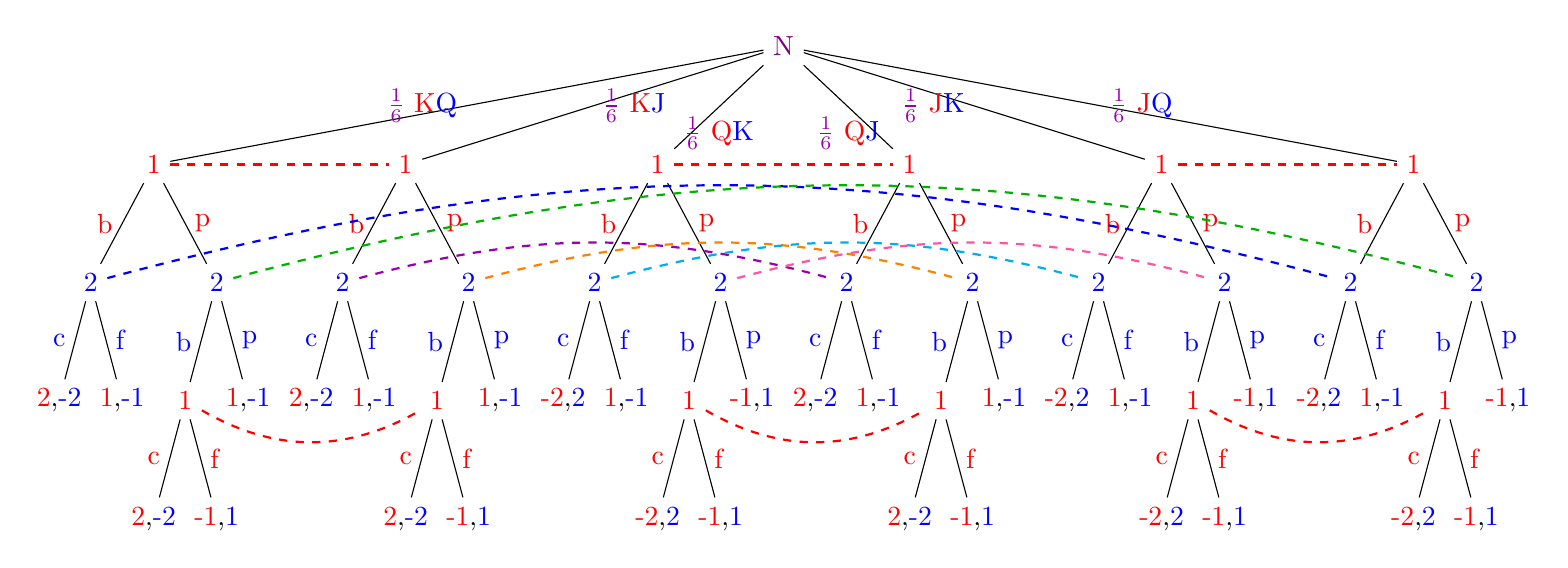
\begin{tikzpicture}[level distance=1.5cm,
  level 1/.style={sibling distance=32mm},
  level 2/.style={sibling distance=16mm},
  level 3/.style={sibling distance=8mm},
  level 4/.style={sibling distance=8mm}]
\node {\nat}
  child {node (KQ) {\one}
    child {node (KQb) {\two}
      child {node { \paystwo{2}{-2} } edge from parent node[left] {\blue{c} }}
      child {node { \paystwo{1}{-1} } edge from parent node[right] {\blue{f} }}
    edge from parent node[left] {\red{b} }}
    child {node (KQp) {\two} 
      child {node (KQpb) { \one }
        child {node { \paystwo{2}{-2} } edge from parent node[left] {\red{c} }}
        child {node { \paystwo{-1}{1} } edge from parent node[right] {\red{f} }}
       edge from parent node[left] {\blue{b} }}
      child {node { \paystwo{1}{-1} } edge from parent node[right] {\blue{p} }}
    edge from parent node[right] {\red{p} }}
  edge from parent node[left] {\purple{$\frac{1}{6}$} \red{K}\blue{Q} }}
  child {node (KJ) {\one}
    child {node (KJb) {\two}
      child {node { \paystwo{2}{-2} } edge from parent node[left] {\blue{c} }}
      child {node { \paystwo{1}{-1} } edge from parent node[right] {\blue{f} }}
    edge from parent node[left] {\red{b} }}
    child {node (KJp) {\two}
      child {node (KJpb) { \one }
        child {node { \paystwo{2}{-2} } edge from parent node[left] {\red{c} }}
        child {node { \paystwo{-1}{1} } edge from parent node[right] {\red{f} }}
      edge from parent node[left] {\blue{b} }}
      child {node { \paystwo{1}{-1} } edge from parent node[right] {\blue{p} }}
    edge from parent node[right] {\red{p} }}
  edge from parent node[right] {\purple{$\frac{1}{6}$} \red{K}\blue{J} }}
  child {node (QK) {\one}
    child {node (QKb) {\two}
      child {node { \paystwo{-2}{2} } edge from parent node[left] {\blue{c} }}
      child {node { \paystwo{1}{-1} } edge from parent node[right] {\blue{f} }}
    edge from parent node[left] {\red{b} }}
    child {node (QKp) {\two}
      child {node (QKpb) { \one }
        child {node { \paystwo{-2}{2} } edge from parent node[left] {\red{c} }}
        child {node { \paystwo{-1}{1} } edge from parent node[right] {\red{f} }}
      edge from parent node[left] {\blue{b} }}
      child {node { \paystwo{-1}{1} } edge from parent node[right] {\blue{p} }}
    edge from parent node[right] {\red{p} }}
  edge from parent node[below] {\purple{$\frac{1}{6}$} \red{Q}\blue{K} }}
  child {node (QJ) {\one}
    child {node (QJb) {\two}
      child {node { \paystwo{2}{-2} } edge from parent node[left] {\blue{c} }}
      child {node { \paystwo{1}{-1} } edge from parent node[right] {\blue{f} }}
    edge from parent node[left] {\red{b} }}
    child {node (QJp) {\two}
      child {node (QJpb) { \one }
        child {node { \paystwo{2}{-2} } edge from parent node[left] {\red{c} }}
        child {node { \paystwo{-1}{1} } edge from parent node[right] {\red{f} }}
      edge from parent node[left] {\blue{b} }}
      child {node { \paystwo{1}{-1} } edge from parent node[right] {\blue{p} }}
    edge from parent node[right] {\red{p} }}
  edge from parent node[below] {\purple{$\frac{1}{6}$} \red{Q}\blue{J} }}
  child {node (JK) {\one}
    child {node (JKb) {\two}
      child {node { \paystwo{-2}{2} } edge from parent node[left] {\blue{c} }}
      child {node { \paystwo{1}{-1} } edge from parent node[right] {\blue{f} }}
    edge from parent node[left] {\red{b} }}
    child {node (JKp) {\two}
      child {node (JKpb) { \one }
        child {node { \paystwo{-2}{2} } edge from parent node[left] {\red{c} }}
        child {node { \paystwo{-1}{1} } edge from parent node[right] {\red{f} }}
      edge from parent node[left] {\blue{b} }}
      child {node { \paystwo{-1}{1} } edge from parent node[right] {\blue{p} }}
    edge from parent node[right] {\red{p} }}
  edge from parent node[left] {\purple{$\frac{1}{6}$} \red{J}\blue{K} }}
  child {node (JQ) {\one}
    child {node (JQb) {\two}
      child {node { \paystwo{-2}{2} } edge from parent node[left] {\blue{c} }}
      child {node { \paystwo{1}{-1} } edge from parent node[right] {\blue{f} }}
    edge from parent node[left] {\red{b} }}
    child {node (JQp) {\two}
      child {node (JQpb) { \one }
        child {node { \paystwo{-2}{2} } edge from parent node[left] {\red{c} }}
        child {node { \paystwo{-1}{1} } edge from parent node[right] {\red{f} }}
      edge from parent node[left] {\blue{b} }}
      child {node { \paystwo{-1}{1} } edge from parent node[right] {\blue{p} }}
    edge from parent node[right] {\red{p} }}
  edge from parent node[right] {\purple{$\frac{1}{6}$} \red{J}\blue{Q} }}
;
\draw[red,dashed,thick] (KQ) -- (KJ);
\draw[red,dashed,thick] (QK) -- (QJ);
\draw[red,dashed,thick] (JK) -- (JQ);
\draw[red,dashed,thick] (KQpb) to[bend right=30] (KJpb);
\draw[red,dashed,thick] (QKpb) to[bend right=30] (QJpb);
\draw[red,dashed,thick] (JKpb) to[bend right=30] (JQpb);
\draw[blue,dashed,thick] (KQb) to[bend left=15] (JQb);
\draw[Green,dashed,thick] (KQp) to[bend left=15] (JQp);
\draw[Purple,dashed,thick] (KJb) to[bend left=15] (QJb);
\draw[orange,dashed,thick] (KJp) to[bend left=15] (QJp);
\draw[cyan,dashed,thick] (QKb) to[bend left=15] (JKb);
\draw[Pink,dashed,thick] (QKp) to[bend left=15] (JKp);
\end{tikzpicture}
}

\begin{tabular}{|c|c|c|}
\hline
\red{$P_1$} & \red{\$} & \red{$\emptyset$} \\ \hline
\red{K}			& 4 & 2 \\ \hline
\red{Q}			& 3 & 3 \\ \hline
\red{J}			& 2 & 4 \\ \hline
\red{Kp}\blue{b}		& 5 & 1 \\ \hline
\red{Qp}\blue{b}	& 3 & 3 \\ \hline
\red{Jp}\blue{b}		& 1 & 5 \\ \hline
\end{tabular}
\hspace{5mm}
\begin{tabular}{|c|c|c|}
\hline
\blue{$P_2$} & \blue{\$} & \blue{$\emptyset$} \\ \hline
\textcolor{cyan}{\textbullet}\blue{K}\red{b}		& 5 & 1 \\ \hline
\textcolor{Pink}{\textbullet}\blue{K}\red{b}		& 5 & 1 \\ \hline
\blue{\textbullet Q}\red{b}					& 3 & 3 \\ \hline
\green{\textbullet}\blue{Q}\red{p}			& 4 & 2 \\ \hline
\purple{\textbullet}\blue{J}\red{b}			& 1 & 5 \\ \hline
\textcolor{orange}{\textbullet}\blue{J}\red{p}	& 2 & 4 \\ \hline
\end{tabular}


You have been provided with correct solutions for \blue{Player 2}.
Complete the solution by filling in results for \red{Player 1} in each table.
You do not need to show the steps that are done per-node (it's recommended that you still work through those steps, but you don't need to write up the results in \LaTeX).
\textbf{Hint:} when calculating the expected utility of an information set, you can check your work by doing it two ways:
first fill in the deviation payoffs and multiply by strategy probabilities;
then find node-utilities and multiply by belief probabilities.
These should give the same answer!

\answer{

\begin{enumerate}[(a)]

\item
Identify the current profile of behavioral strategies.

\begin{tabular}{|c|c|c|}
\hline
\red{$P_1$} & \red{\$} & \red{$\emptyset$} \\ \hline
\red{K}			& $\frac{2}{3}$ & $\frac{1}{3}$ \\ \hline
\red{Q}			& $\frac{1}{2}$ & $\frac{1}{2}$ \\ \hline
\red{J}			& $\frac{1}{3}$ & $\frac{2}{3}$ \\ \hline
\red{Kp}\blue{b}		& $\frac{5}{6}$ & $\frac{1}{6}$ \\ \hline
\red{Qp}\blue{b}	& $\frac{1}{2}$ & $\frac{1}{2}$ \\ \hline
\red{Jp}\blue{b}		& $\frac{1}{6}$ & $\frac{5}{6}$ \\ \hline
\end{tabular}
\hspace{5mm}
\begin{tabular}{|c|c|c|}
\hline
\blue{$P_2$} & \blue{\$} & \blue{$\emptyset$} \\ \hline
\textcolor{cyan}{\textbullet}\blue{K}\red{b}		& $\frac{5}{6}$ & $\frac{5}{6}$ \\ \hline
\textcolor{Pink}{\textbullet}\blue{K}\red{b}		& $\frac{5}{6}$ & $\frac{5}{6}$ \\ \hline
\blue{\textbullet Q}\red{b}					& $\frac{1}{2}$ & $\frac{1}{2}$ \\ \hline
\green{\textbullet}\blue{Q}\red{p}			& $\frac{2}{3}$ & $\frac{1}{3}$ \\ \hline
\purple{\textbullet}\blue{J}\red{b}			& $\frac{1}{6}$ & $\frac{5}{6}$ \\ \hline
\textcolor{orange}{\textbullet}\blue{J}\red{p}	& $\frac{1}{3}$ & $\frac{2}{3}$ \\ \hline
\end{tabular}



\item
Find conditional beliefs at each information set using those probabilities.

\begin{tabular}{|c|c|c|}
\hline
\red{$P_1$} & \red{\$} & \red{$\emptyset$} \\ \hline
\red{K}			& $\frac{1}{2}$ & $\frac{1}{2}$ \\ \hline
\red{Q}			& $\frac{1}{2}$ & $\frac{1}{2}$ \\ \hline
\red{J}			& $\frac{1}{2}$ & $\frac{1}{2}$ \\ \hline
\red{Kp}\blue{b}		& $\frac{2}{3}$ & $\frac{1}{3}$ \\ \hline
\red{Qp}\blue{b}	& $\frac{5}{7}$ & $\frac{2}{7}$ \\ \hline
\red{Jp}\blue{b}		& $\frac{5}{9}$ & $\frac{4}{9}$ \\ \hline
\end{tabular}
\hspace{5mm}
\begin{tabular}{|c|c|c|}
\hline
\blue{$P_2$} & \blue{\$} & \blue{$\emptyset$} \\ \hline
\textcolor{cyan}{\textbullet}\blue{K}\red{b}		& $\frac{3}{5}$ & $\frac{2}{5}$ \\ \hline
\textcolor{Pink}{\textbullet}\blue{K}\red{b}		& $\frac{3}{7}$ & $\frac{4}{7}$ \\ \hline
\blue{\textbullet Q}\red{b}					& $\frac{2}{3}$ & $\frac{1}{3}$ \\ \hline
\green{\textbullet}\blue{Q}\red{p}			& $\frac{1}{3}$ & $\frac{2}{3}$ \\ \hline
\purple{\textbullet}\blue{J}\red{b}			& $\frac{4}{7}$ & $\frac{3}{7}$ \\ \hline
\textcolor{orange}{\textbullet}\blue{J}\red{p}	& $\frac{2}{5}$ & $\frac{3}{5}$ \\ \hline
\end{tabular}



\item
Find the deviation payoff for each action and the expected utility of each information set.

\begin{tabular}{|c|c|c|c|}
\hline
\red{$P_1$} & \red{\$} & \red{$\emptyset$} & \red{IS} \\ \hline
\red{K}			& $\frac{4}{3}$ & $\frac{5}{4}$ & $\frac{47}{36}$ \\ \hline
\red{Q}			& $-\frac{1}{6}$ & $-\frac{7}{24}$ & $-\frac{11}{48}$ \\ \hline
\red{J}			& $-1$ & $-\frac{9}{8}$ & $-\frac{13}{12}$ \\ \hline
\red{Kp}\blue{b}		& $2$ & $-1$ & $\frac{3}{2}$ \\ \hline
\red{Qp}\blue{b}	& $-\frac{6}{7}$ & $-1$ & $-\frac{13}{14}$ \\ \hline
\red{Jp}\blue{b}		& $-2$ & $-1$ & $-\frac{7}{6}$ \\ \hline
\end{tabular}
\hspace{5mm}
\begin{tabular}{|c|c|c|c|}
\hline
\blue{$P_2$} & \blue{\$} & \blue{$\emptyset$} & \blue{IS} \\ \hline
\textcolor{cyan}{\textbullet}\blue{K}\red{b}		& $2$			& $-1$		& $\frac{3}{2}$		\\ \hline
\textcolor{Pink}{\textbullet}\blue{K}\red{b}		& $\frac{55}{42}$	& 1			& $\frac{317}{252}$	\\ \hline
\blue{\textbullet Q}\red{b}					& $-\frac{2}{3}$		& $-1$		& $-\frac{5}{6}$		\\ \hline
\green{\textbullet}\blue{Q}\red{p}			& $\frac{5}{18}$		& $\frac{1}{3}$	& $\frac{8}{27}$		\\ \hline
\purple{\textbullet}\blue{J}\red{b}			& $-2$			& $-1$		& $-\frac{7}{6}$		\\ \hline
\textcolor{orange}{\textbullet}\blue{J}\red{p}	& $-\frac{9}{10}$	& $-1$		& $-\frac{29}{30}$	\\ \hline
\end{tabular}



\item
Find the probability-weighted gain for each action at each information set.

\begin{tabular}{|c|c|c|}
\hline
\red{$P_1$} & \red{\$} & \red{$\emptyset$} \\ \hline
\red{K}			& $\frac{1}{108}$ & $0$ \\ \hline
\red{Q}			& $\frac{1}{48}$ & $0$ \\ \hline
\red{J}			& $\frac{1}{36}$ & $0$ \\ \hline
\red{Kp}\blue{b}		& $\frac{1}{3}$ & $0$ \\ \hline
\red{Qp}\blue{b}	& $\frac{1}{56}$ & $0$ \\ \hline
\red{Jp}\blue{b}		& $0$ & $\frac{1}{24}$ \\ \hline
\end{tabular}
\hspace{5mm}
\begin{tabular}{|c|c|c|}
\hline
\blue{$P_2$} & \blue{\$} & \blue{$\emptyset$} \\ \hline
\textcolor{cyan}{\textbullet}\blue{K}\red{b}		& $\frac{5}{72}$ & 0 \\ \hline
\textcolor{Pink}{\textbullet}\blue{K}\red{b}		& $\frac{13}{1296}$ & 0 \\ \hline
\blue{\textbullet Q}\red{b}					& $\frac{1}{36}$ & 0 \\ \hline
\green{\textbullet}\blue{Q}\red{p}			& 0 & $\frac{1}{162}$ \\ \hline
\purple{\textbullet}\blue{J}\red{b}			& 0 & $\frac{7}{216}$ \\ \hline
\textcolor{orange}{\textbullet}\blue{J}\red{p}	& $\frac{1}{108}$ & 0 \\ \hline
\end{tabular}



\item
Find the new strategy profile by updating the cumulative gains and normalizing.

\begin{tabular}{|c|c|c|}
\hline
\red{$P_1$} & \red{\$} & \red{$\emptyset$} \\ \hline
\red{K}			& $0.6672$ & $0.3328$ \\ \hline
\red{Q}			& $0.5017$ & $0.4983$ \\ \hline
\red{J}			& $0.3364$ & $0.6636$ \\ \hline
\red{Kp}\blue{b}		& $0.8421$ & $0.1579$ \\ \hline
\red{Qp}\blue{b}	& $0.5014$ & $0.4985$ \\ \hline
\red{Jp}\blue{b}		& $0.1655$ & $0.8345$ \\ \hline
\end{tabular}
\hspace{5mm}
\begin{tabular}{|c|c|c|}
\hline
\blue{$P_2$} & \blue{\$} & \blue{$\emptyset$} \\ \hline
\textcolor{cyan}{\textbullet}\blue{K}\red{b}		& .8352 & .1648 \\ \hline
\textcolor{Pink}{\textbullet}\blue{K}\red{b}		& .8336 & .1664 \\ \hline
\blue{\textbullet Q}\red{b}					& .5023 & .4977 \\ \hline
\green{\textbullet}\blue{Q}\red{p}			& .6660 & .3340 \\ \hline
\purple{\textbullet}\blue{J}\red{b}			& .1658 & .8342 \\ \hline
\textcolor{orange}{\textbullet}\blue{J}\red{p}	& .3344 & .6656 \\ \hline
\end{tabular}

\end{enumerate}

}



\end{document}